% Figure 1a -- the consent pipeline on a Shopify storefront, with the sandbox blind spot.
% Final printed size: 120 mm x 79 mm (Figure 1 top-left; 1b sits to its right, 1c below).
% Every element is taken from ../../notes/mechanism.md (sections 1, 2.1, 2.4, 2.5, 3).
% Encoding: solid light grey strip = runs in the page's main thread; 45-degree hatch = runs in a
% Shopify sandbox (web worker or sandboxed iframe); accent red = the blind spot, nothing else.
\documentclass[tikz,border=2pt]{standalone}
% schematic_style.tex -- shared style for every TikZ schematic panel (Fig 1a, 2a-2d).
% Binding source: ../../FIGURE_PLAN.md (style guide). Change colours here only.
% one sans face in BOTH engines (matplotlib panels use Arial too); Courier New for code (review: typography)
\usepackage{fontspec}\setmainfont{Arial}\setsansfont{Arial}\setmonofont{Courier New}
\renewcommand{\familydefault}{\sfdefault}
\usepackage{xcolor}
\usetikzlibrary{arrows.meta,calc,patterns.meta,shapes.geometric,positioning}

% ---- fixed vendor colours (FIGURE_PLAN.md, validated categorical order) ----
\definecolor{vGoogle}{HTML}{2A78D6}
\definecolor{vTikTok}{HTML}{EB6834}
\definecolor{vMeta}{HTML}{1BAF7A}
\definecolor{vPinterest}{HTML}{EDA100}
\definecolor{vSnap}{HTML}{E87BA4}
\definecolor{vMicrosoft}{HTML}{008300}
\definecolor{vOther}{HTML}{4A3AA7}
% ---- neutrals, arms (shape + grey, never hue), accent ----
\definecolor{ink}{HTML}{0B0B0B}      % text; Default arm
\definecolor{greyD}{HTML}{52514E}    % box outlines; Decline + Repeat arms
\definecolor{greyM}{HTML}{8A8984}    % sandbox hatch; GPC arm; secondary text
\definecolor{greyL}{HTML}{DEDDD9}    % main-thread origin (solid light grey)
\definecolor{greyXL}{HTML}{F3F2EF}   % faint container fill
\definecolor{accent}{HTML}{D03B3B}   % ONLY meaning: consent failed / blind spot
\colorlet{tbdgrey}{greyM}

% ---- sizes: 7 pt body, 10 pt bold panel letter ----
\newcommand{\fsBody}{\fontsize{7}{8.2}\selectfont}
\newcommand{\fsLetter}{\fontsize{10}{12}\selectfont\bfseries}
\newcommand{\fsTitle}{\fontsize{8}{9.6}\selectfont\bfseries}   % panel titles: 8 pt bold, as in the matplotlib panels (review FIG-20)

\tikzset{
  x=1mm, y=1mm,
  every picture/.style={line width=0.4pt},
  every node/.style={font=\fsBody, text=ink, inner sep=0.6mm},
  % arrows
  arr/.style={-{Stealth[length=1.5mm,width=1.1mm]}, draw=ink, line width=0.45pt},
  arrg/.style={-{Stealth[length=1.5mm,width=1.1mm]}, draw=greyD, line width=0.45pt},
  % boxes
  box/.style={draw=greyD, fill=white, rounded corners=0.7mm, line width=0.4pt},
  mainthread/.style={fill=greyL},
  sandbox/.style={pattern={Lines[angle=45,distance=1.25pt,line width=0.35pt]}, pattern color=greyM},
  % text helpers
  lbl/.style={align=left, anchor=north west, inner sep=0pt},
  lblc/.style={align=center, inner sep=0pt},
  note/.style={align=left, inner sep=0pt, text=greyD},
  panelletter/.style={font=\fsLetter, anchor=north west, inner sep=0pt},
  % arm markers (FIGURE_PLAN: Default filled circle #0b0b0b; Decline open square #52514e;
  % GPC filled triangle #8a8984; Repeat/validation open diamond #52514e)
  mDefault/.style={circle, fill=ink, draw=ink, inner sep=0pt, minimum size=2.1mm},
  mDecline/.style={rectangle, fill=white, draw=greyD, line width=0.7pt, inner sep=0pt, minimum size=1.85mm},
  mGPC/.style={regular polygon, regular polygon sides=3, fill=greyM, draw=greyM, inner sep=0pt, minimum size=2.7mm},
  mRepeat/.style={diamond, fill=white, draw=greyD, line width=0.7pt, inner sep=0pt, minimum size=2.4mm},
}

% vendor chip: \chip{vTikTok}  (small filled square; identity is always also named in text)
\newcommand{\chip}[1]{\tikz[baseline=-0.1mm]\fill[#1] (0,0) rectangle (1.7mm,1.7mm);}
% origin swatches for legends, same encoding as the data figures (3c)
\newcommand{\swMain}{\tikz[baseline=-0.1mm]\draw[greyD,fill=greyL,line width=0.3pt] (0,0) rectangle (3.2mm,1.9mm);}
\newcommand{\swSand}{\tikz[baseline=-0.1mm]\draw[greyD,line width=0.3pt,pattern={Lines[angle=45,distance=1.25pt,line width=0.35pt]},pattern color=greyM] (0,0) rectangle (3.2mm,1.9mm);}
% inline arm markers for text
\newcommand{\mkDefault}{\tikz[baseline=-0.75mm]\node[mDefault]{};}
\newcommand{\mkDecline}{\tikz[baseline=-0.75mm]\node[mDecline]{};}
\newcommand{\mkGPC}{\tikz[baseline=-0.95mm]\node[mGPC]{};}
\newcommand{\mkRepeat}{\tikz[baseline=-0.75mm]\node[mRepeat]{};}
\newcommand{\blindstar}{\tikz[baseline=-0.35mm]\node[star,star points=5,star point ratio=2.3,fill=accent,inner sep=0pt,minimum size=2.3mm]{};}

% Exact final size: standalone adds a 2pt border on every side, so the drawn
% bounding box is (W - 4pt) x (H - 4pt) and the PDF is exactly W x H.
\newcommand{\panelsize}[2]{\path[use as bounding box] (0,0) rectangle ($(#1,#2)-(4pt,4pt)$);}
\newcommand{\panelletter}[2]{\node[panelletter] at ($(0,#2)-(0,4pt)$) {#1};}

% numbers.tex -- GENERATED by make_numbers.py; do not edit by hand.
% Placeholders (\nTBD) are filled when the listed source file exists.
\providecommand{\nTBD}{{\color{tbdgrey}[n\,=\,?]}}
\newcommand{\nTrancoList}{L5PZ4}% funnel.json:tranco_list_id
\newcommand{\nTranco}{200,000}% funnel.json:top_n
\newcommand{\nResolved}{181,310}% funnel.json:domains_with_any_A_record
\newcommand{\nDNSShopify}{2,634}% funnel.json:dns_flagged_shopify
\newcommand{\nDrawn}{1,518}% funnel.json:drawn_for_verification
\newcommand{\nCensus}{902}% sum drawn_n over buckets with sampling_fraction 1
\newcommand{\nRandomDrawn}{616}% drawn_n, randomly sampled bucket
\newcommand{\nRandomFrame}{1,732}% flagged_N, randomly sampled bucket
\newcommand{\nHTTPok}{1,491}% funnel.json:http_200
\newcommand{\nStorefront}{1,438}% funnel.json:verified_live_online_store
\newcommand{\nAfterContent}{1,424}% funnel.json:after_content_exclusions
\newcommand{\nWithProduct}{1,407}% funnel.json:with_product_url
\newcommand{\nSample}{1,400}% funnel.json:sample_after_dedupe
\newcommand{\nCreator}{34}% rows in creator_stratum.csv
\newcommand{\nCaptured}{1,362}% analysis/crawl_funnel.json:captured_all_arms
\newcommand{\nCreatorCaptured}{34}% analysis/crawl_funnel.json:captured_creator
\newcommand{\nExclLive}{80}% analysis/crawl_funnel.json:funnel_excl.drawn_to_live
\newcommand{\nExclSample}{38}% analysis/crawl_funnel.json:funnel_excl.live_to_sample
\newcommand{\nExclCaptured}{38}% analysis/crawl_funnel.json:funnel_excl.sample_to_captured
\newcommand{\nRepeatPlanned}{287}% analysis/crawl_funnel.json:repeat_planned
\newcommand{\nRepeatOk}{274}% analysis/crawl_funnel.json:repeat_main_ok
\newcommand{\nBravePlanned}{100}% analysis/crawl_funnel.json:brave_planned
\newcommand{\nBraveOk}{99}% analysis/crawl_funnel.json:brave_ok
\newcommand{\pRegionAllowed}{82}% analysis/outputs/stats.json:fig1b.region_allowed.p

% box with an origin strip on its left edge: \obox{x1}{y1}{x2}{y2}{mainthread|sandbox}
\newcommand{\obox}[5]{%
  \draw[box] (#1,#2) rectangle (#3,#4);
  \begin{scope}\clip[rounded corners=0.7mm] (#1,#2) rectangle (#3,#4);
    \fill[#5] (#1,#2) rectangle (#1+2.2,#4);\end{scope}
  \draw[greyD, rounded corners=0.7mm] (#1,#2) rectangle (#3,#4);}
\begin{document}
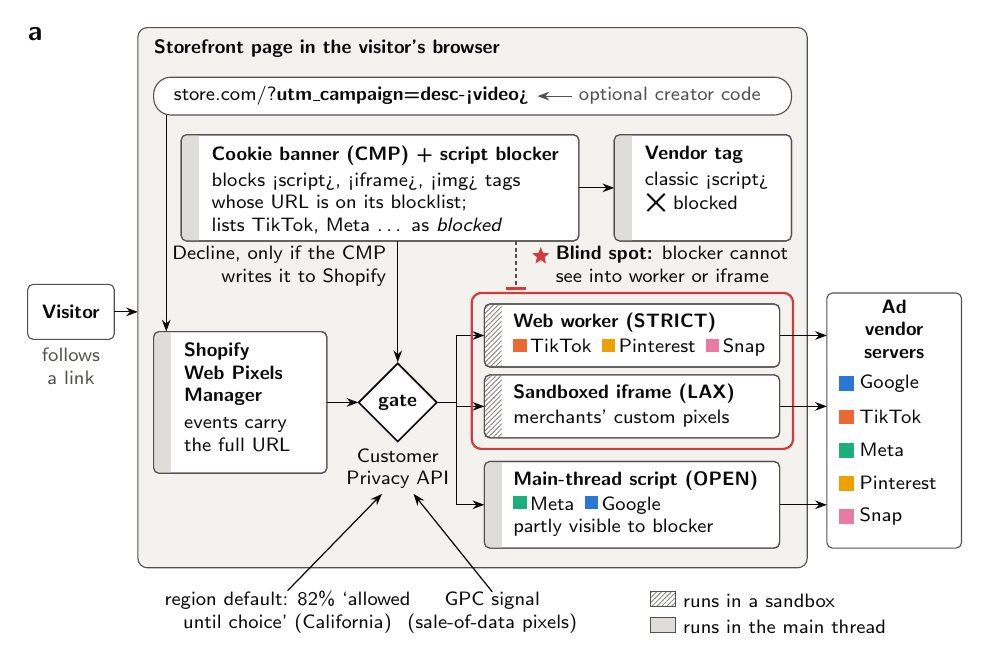
\begin{tikzpicture}
\def\W{120}\def\H{79}
\panelsize{\W}{\H}
\panelletter{a}{\H}

% ------------------------------------------------------------------ visitor
\draw[box] (0,38) rectangle (11,45);
\node[lblc] at (5.5,41.5) {\textbf{Visitor}};
\node[note, align=center] at (5.5,34.6) {follows\\a link};
\draw[arr] (11,41.5) -- (14,41.5);

% ------------------------------------------------------------------ storefront page (browser)
\draw[draw=greyD, fill=greyXL, rounded corners=1.2mm] (14,9) rectangle (99,77.6);
\node[lbl] at (16,76.1) {\textbf{Storefront page in the visitor's browser}};
% address bar with an optional creator code
\draw[draw=greyD, fill=white, rounded corners=2.2mm] (16,66.5) rectangle (97,71.3);
\node[anchor=west, inner sep=0pt] (url) at (18.5,68.9) {store.com/?\textbf{utm\_campaign=desc-<video>}};
\draw[arrg] ([xshift=5.4mm]url.east) -- ([xshift=1.0mm]url.east);
\node[anchor=west, inner sep=0pt, text=greyD] at ([xshift=6.2mm]url.east) {optional creator code};

% ------------------------------------------------------------------ lane 1: CMP (main thread)
\obox{19.5}{50.5}{70}{64}{mainthread}
\node[lbl] at (23.3,62.6) {\textbf{Cookie banner (CMP) + script blocker}\\[0.35mm]
  blocks <script>, <iframe>, <img> tags\\ whose URL is on its blocklist;\\ lists TikTok, Meta \ldots\ as \emph{blocked}};
\draw[arr] (70,57.25) -- (74.5,57.25);
\obox{74.5}{50.5}{97}{64}{mainthread}
\node[lbl] at (78.3,62.6) {\textbf{Vendor tag}\\[0.35mm] classic <script>};
\draw[ink, line width=0.7pt] (78.7,54.3) -- (80.9,56.5) (78.7,56.5) -- (80.9,54.3);
\node[anchor=west, inner sep=0pt] at (81.9,55.4) {blocked};

% ------------------------------------------------------------------ lane 2: Shopify Web Pixels Manager
\obox{16}{21}{38}{39}{mainthread}
\node[lbl] at (19.8,37.6) {\textbf{Shopify}\\ \textbf{Web Pixels}\\ \textbf{Manager}\\[0.5mm] events carry\\ the full URL};
% the page URL (with any creator code) enters every event: URL -> Web Pixels Manager
\draw[arr] (17.6,66.5) -- (17.6,39);
\draw[arr] (38,30) -- (42,30);

% the gate
\node[diamond, draw=ink, fill=white, line width=0.6pt, minimum size=10mm, inner sep=0pt] (gate) at (47,30) {\textbf{gate}};
\node[lblc, anchor=north] (cpapi) at (47,24.2) {Customer\\ Privacy API};

% containers: \cbox{y-bottom}{height}{origin style}{title}{line 2}{name}
\newcommand{\cbox}[6]{%
  \obox{58}{#1}{95.5}{#1+#2}{#3}
  \node[lbl] at (61.6,#1+#2-1.1) {\textbf{#4}\\[0.3mm] #5};
  \coordinate (#6) at (95.5,#1+#2/2);
  \coordinate (#6in) at (58,#1+#2/2);}
\cbox{34.5}{8}{sandbox}{Web worker (STRICT)}{\chip{vTikTok}\,TikTok\enspace\chip{vPinterest}\,Pinterest\enspace\chip{vSnap}\,Snap}{w}
\cbox{25.5}{8}{sandbox}{Sandboxed iframe (LAX)}{merchants' custom pixels}{f}
\cbox{11.5}{11}{mainthread}{Main-thread script (OPEN)}{\chip{vMeta}\,Meta\enspace\chip{vGoogle}\,Google\\ partly visible to blocker}{o}

% gate -> bus -> containers
\draw[ink, line width=0.45pt] (gate.east) -- (54.5,30);
\draw[ink, line width=0.45pt] (54.5,17) -- (54.5,38.5);
\draw[arr] (54.5,38.5) -- (win);
\draw[arr] (54.5,29.5) -- (fin);
\draw[arr] (54.5,17) -- (oin);

% the blind spot (the ONE use of the accent colour)
\draw[accent, line width=0.8pt, rounded corners=1.2mm] (56.4,24.1) rectangle (97.2,43.9);

% ------------------------------------------------------------------ how the CMP can reach lane 2
% (1) script blocker: its reach ends at the sandbox boundary
\draw[greyD, line width=0.55pt, dash pattern=on 1.4pt off 1pt, -{Bar[width=2.6mm,line width=1.1pt,color=accent]}] (62,50.5) -- (62,44.3);
\node[anchor=north west, inner sep=0pt] at (64,49.8) {\blindstar};
\node[lbl] at (67,49.9) {\textbf{Blind spot:} blocker cannot\\ see into worker or iframe};
% (2) Decline reaches the gate only through Shopify
\draw[arr] (47,50.5) -- (gate.north);
\node[align=right, anchor=north east, inner sep=0pt] at (45.6,49.9) {Decline, only if the CMP\\ writes it to Shopify};

% ------------------------------------------------------------------ gate inputs from outside the page
\node[lblc, anchor=south] (reg) at (33,0.6) {region default: \pRegionAllowed\% `allowed\\ until choice' (California)};
\node[lblc, anchor=south] (gpc) at (59,0.6) {GPC signal\\ (sale-of-data pixels)};
\draw[arr] (reg.north) -- ([xshift=-2mm,yshift=-0.6mm]cpapi.south);
\draw[arr] (gpc.north) -- ([xshift=2mm,yshift=-0.6mm]cpapi.south);

% ------------------------------------------------------------------ vendors
\draw[box] (101.5,11.5) rectangle (118.6,43.9);
\node[lblc, anchor=north] at (110.05,43.1) {\textbf{Ad}\\ \textbf{vendor}\\ \textbf{servers}};
\foreach \c/\n [count=\i] in {vGoogle/Google,vTikTok/TikTok,vMeta/Meta,vPinterest/Pinterest,vSnap/Snap}{
  \fill[\c] (103,{31.4-(\i-1)*4.2}) rectangle ++(1.9,1.9);
  \node[anchor=west, inner sep=0pt] at (105.6,{32.35-(\i-1)*4.2}) {\n};}
\draw[arr] (w) -- (w -| 101.5,0);
\draw[arr] (f) -- (f -| 101.5,0);
\draw[arr] (o) -- (o -| 101.5,0);

% ------------------------------------------------------------------ legend
\node[lbl, anchor=south west] at (79,0.6) {\swSand\ runs in a sandbox\\[0.4mm] \swMain\ runs in the main thread};
\end{tikzpicture}
\end{document}
